\newpage

\makeatletter
\newcommand{\AlgoResetCount}{\renewcommand{\@ResetCounterIfNeeded}{\setcounter{AlgoLine}{0}}}
\newcommand{\AlgoNoResetCount}{\renewcommand{\@ResetCounterIfNeeded}{}}
\newcounter{AlgoSavedLineCount}
\newcommand{\AlgoSaveLineCount}{\setcounter{AlgoSavedLineCount}{\value{AlgoLine}}}
\newcommand{\AlgoRestoreLineCount}{\setcounter{AlgoLine}{\value{AlgoSavedLineCount}}}
\makeatother



\appendix

\section{Computational Costs of Experiments}
\label{appendix:computationalcosts}
\begin{table}[h]
    \small
    \centering
    \begin{tabular}{l|cccc}
    \toprule
    \textbf{Experiment Type} & \textbf{Experiment Name} & \textbf{Target Claim} & \textbf{Section} & \textbf{GPU Hours} \\
   
    \midrule 
    \multirow{2}{*}{\shortstack[l]{Reproducibility\\ Study}} 
    & \ref{rsexp1}  & \ref{claim1} & \ref{sssec:result1} & 9\\
    & \ref{rsexp21}  & \ref{claim2}  & \ref{exampleimpresult} & 3 \\
    & \ref{rsexp22}  & \ref{claim2}  & \ref{exampleimpresult} & 22 \\
    & \ref{rsexp23}  & \ref{claim2}  & \ref{exampleimpresult} & 2 \\
    & \ref{rsexp31} (GS)  & \ref{claim3}  & \ref{section:result3} & 5\\
    & \ref{rsexp31} (IG)  & \ref{claim3}  & \ref{section:result3} & 8\\
    & \ref{rsexp32} (GS)  & \ref{claim3}  & \ref{section:result3} & 10 \\
    & \ref{rsexp32} (IG)  & \ref{claim3}  & \ref{section:result3} & 28 \\
    & \ref{rsexp4}  & \ref{claim4}  & \ref{section:result4} & 3\\
    % \cline{2-5}
    \midrule
    \multirow{3}{*}{\shortstack[l]{Additional\\ Experiments}} 
      & \ref{aexp1} &  \ref{claim1} & \ref{sec:result1extra} & 4 \\
      & \ref{aexp2}  & \ref{claim2} & \ref{sec:result2extra} & 8 \\
      & \ref{aexp3}  & \ref{claim3}  & \ref{sec:result3extra} & 8 \\
      
    \midrule

    \end{tabular}
    \caption{Computational Cost for each experiment, measured in GPU hours.}
    \label{table:computational_costs}
\end{table}

The conducted \textbf{Reproducibility Study Experiments (rs-exp)} of this work are:
\begin{enumerate}[labelindent=\parindent,leftmargin=*, label=\textbf{rs-exp \arabic*},noitemsep,topsep=0pt]
    \itemsep0em
    \item\label{rsexp1} Consistency Check of label-Free Feature Importance.
    \item\label{rsexp2} Consistency Check of label-free Example Importance.
        \begin{enumerate}[labelindent=\parindent,leftmargin=*, label=\textbf{rs-exp2 \arabic*},noitemsep,topsep=0pt]
        \itemsep0em
        \item\label{rsexp21} MNIST.
        \item\label{rsexp22} ECG5000.
        \item\label{rsexp23} CIFAR10.
        \end{enumerate}
    \item\label{rsexp3} Challenging authors' assumptions with disentangled VAEs using Integrated Gradients (IG) \& Gradient Shap (GS).
    \begin{enumerate}[labelindent=\parindent,leftmargin=*, label=\textbf{rs-exp3 \arabic*},noitemsep,topsep=0pt]
    \itemsep0em
    \item\label{rsexp31} MNIST.
    \item\label{rsexp32} dSprites.
    \end{enumerate}
    \item\label{rsexp4} Comparing the Explainability Representations from Different Pretext Tasks. 
\end{enumerate}

\vspace{+2mm}

The conducted \textbf{Additional Experiments (a-exp)} of this work are:
\begin{enumerate}[labelindent=\parindent,leftmargin=*, label=\textbf{a-exp \arabic*},noitemsep,topsep=0pt]
    \itemsep0em
    \item\label{aexp1} \nameref{sec:result1extra}
    \item\label{aexp2} \nameref{sec:result2extra}
    \item\label{aexp3}  Challenging the Generalizability of \ref{claim3} with Attribution Priors on MNIST
\end{enumerate}

\section{Label Free Feature Importance}

\subsection{Graph Explainability}
\label{appendix:graphexplain}

\subsubsection{Model}
\label{sssec:graphmodel}
Since we want to explain the graph in a label-free unsupervised setting, we choose to use a Variational Graph Autoencoder (VGAE) \citep{graphvae}. Table \ref{tab:graphtable} describes the architecture of the model. We perform an edge-link prediction task on the Cora citation dataset. We train the VGAE to minimize the objective:
\begin{align*}
\mathcal{L} = \mathbb{E}_{q(Z|X,A)}[\log p(A|Z)] - KL[q(Z|X,A)||p(Z)]
\end{align*}
where $A$ is the adjacency matrix, $q(Z|X,A)$ is the distribution parameterized by the inference model of 2-layer GCN. $p(Z)$ is the Gaussian prior associated with $\mathcal{N}(0,I)$ and $KL$ is the KL-divergence. We train for 200 epochs with patience 10 by using Pytorch's Adam optimizer with a learning rate = .01.
\begin{table}[h]
    \small
    \centering
    \begin{tabular}{l|cccc}
    \toprule
    \textbf{Component} & \textbf{Layer Type} & \textbf{Hyperparameters} & \textbf{Act. Func} \\
    \midrule 
    \multirow{2}{*}{Encoder} & GraphConv & I/P Feats:1433 ; O/P Feats:32 & ReLU \\
    & &I/P Feats:32 ; O/P Feats:16 & ReLU \\
    \midrule
    \multirow{3}{*}{\shortstack[l]{Reparameterisation\\ Trick}}&  & The output of encoder contains $\mu$ and log$\sigma$. \\
   & & The latent representation is then generated via & \\
      & &  $h = \mu(x)+ \sigma(x)\odot\epsilon, \epsilon \sim \mathcal{N}(0,1)$ \\
    \midrule
    Decoder & & Inner Product Decoder & Sigmoid \\
    \bottomrule
    \end{tabular}
    \caption{Variational Graph Autoencoder Architecture. The last column denotes the activation function used. I/P Feats means Input Features. O/P Feats means output features.}
    \label{tab:graphtable}
\end{table}

\vspace{-3mm}
\subsubsection{Feature Importance}
As a baseline, we use an unconnected graph, $A=0$. In the case of images for the MNIST experiment, we mask important pixels by blackening them. In the case of a graph, we mask important nodes, by isolating them. Algorithm \ref{algograph} summarises steps to compute the feature importance of nodes. 

\begin{algorithm}
  \KwData{Undirected Graph $\mathcal{G}=(\mathcal{V}, \mathcal{E})$ and its adjacency matrix $A$ with $N= |\mathcal{V}|$ nodes. Black-box $f : \mathcal{X}\rightarrow \mathcal{H}$,  Feature importance method $a_i(\cdot,\cdot):\mathcal{A(\mathcal{H}^\mathcal{G}})\times\mathcal{G}\rightarrow \mathbb{R}^N$.}
  \KwResult{Label-Free Feature Importance for nodes $b_i(f, \mathcal{G})$. }
  Convert black-box model $f$ to a model that is usable for captum attribution method \citep{captumaigraph} \;
  Compute \& normalize node attributions of size $|\mathcal{V}|$  \;
  Apply the Mask \;
  Calculate latent shift \;
  Repeat steps 1-3 for different rates of perturbation to induce while masking \;
  \caption{Label Free Feature Importance for Graph}
  \label{algograph}
\end{algorithm}


\subsubsection{Result Discussion}The work \citep{gnnpaper} corroborates our finding that the feature attribution methods are not the right indicator for explaining graphs. The issue of gradient saturation worsens for discrete inputs such as graph adjacency matrices. Future work in this direction can address two issues: (1) Currently, the focus is on explaining graphs for tasks such as node classification. We need a more robust, generalized solution that explains a particular latent representation of the graph, and which graph's attributes (nodes, edges, or subgraphs) are influential. (2) Development of a framework for the previous issue. Appendix section A of \citep{gnnpaper} also addresses the issues we faced while computing important nodes for a particular latent representation. They discuss a 'workaround' to use single-instance explanations to explain a multi-instance explanation (latent representation in our case).  We implemented that in our code base. 


\subsection{Changes in masking and baseline inputs}
\label{section:3_approaches}
We redefine the masking and baseline inputs for the experiments on MNIST using the following approaches:

\vspace{-3mm}
\subsubsection{Change in masking} \label{sssec:changemasking} In the original experiment, the variable $m$ is set to 0 or 1 depending on whether the feature $x_i$ to mask is important ($x_i$ is important when its score is in the top $M$ values as calculated by attribution methods). In the new case, considering a feature pixel $x_i$ and a feature map $x$, we do the masking as follows:

\begin{algorithmic}
\STATE $m \gets 0$
\IF {$x_i$ is an important pixel} 
  \STATE $m_i\gets (1-x_i)/\max(x)$
\ELSE
    \STATE $m_i\gets 1$  
\ENDIF 
\end{algorithmic}

Instead of completely zeroing out an important pixel, we set the mask to a value inversely proportional to its importance. 

\subsubsection{Change in baseline} When we assign blame to a certain cause, we consider the absence of the cause as a baseline for comparing outcomes. In the original experiment, a black image is used as the baseline $\Bar{x}$. Instead of setting all pixels of $\Bar{x}$ to 0, we set the pixel $\Bar{x_i}$ as follows (consider $x$ to be the input image with $x_i$ being its feature pixel): 
\begin{itemize}
    \item We do masking as Appendix Section \ref{sssec:changemasking} and set the baseline image pixels to:
     \begin{align} \label{eqn:app2}
         \Bar{x_i} = (1-x_i)/\max(x)
     \end{align}
  
    \item To the above extension, we also add noise to the baseline image:
     \begin{align} \label{eqn:app3}
         \Bar{x_i} = \mathcal{N}(0,1)*(1-x_i)/\max(x)
     \end{align}
\end{itemize}

\begin{figure*}[h]
\centering
\begin{subfigure}[b]{0.32\linewidth}
\includegraphics[width=\textwidth]{images/feature_imp/approach1.png}
\caption{Change in mask variable}\label{fig:approach1}
\end{subfigure}
\begin{subfigure}[b]{0.32\linewidth}
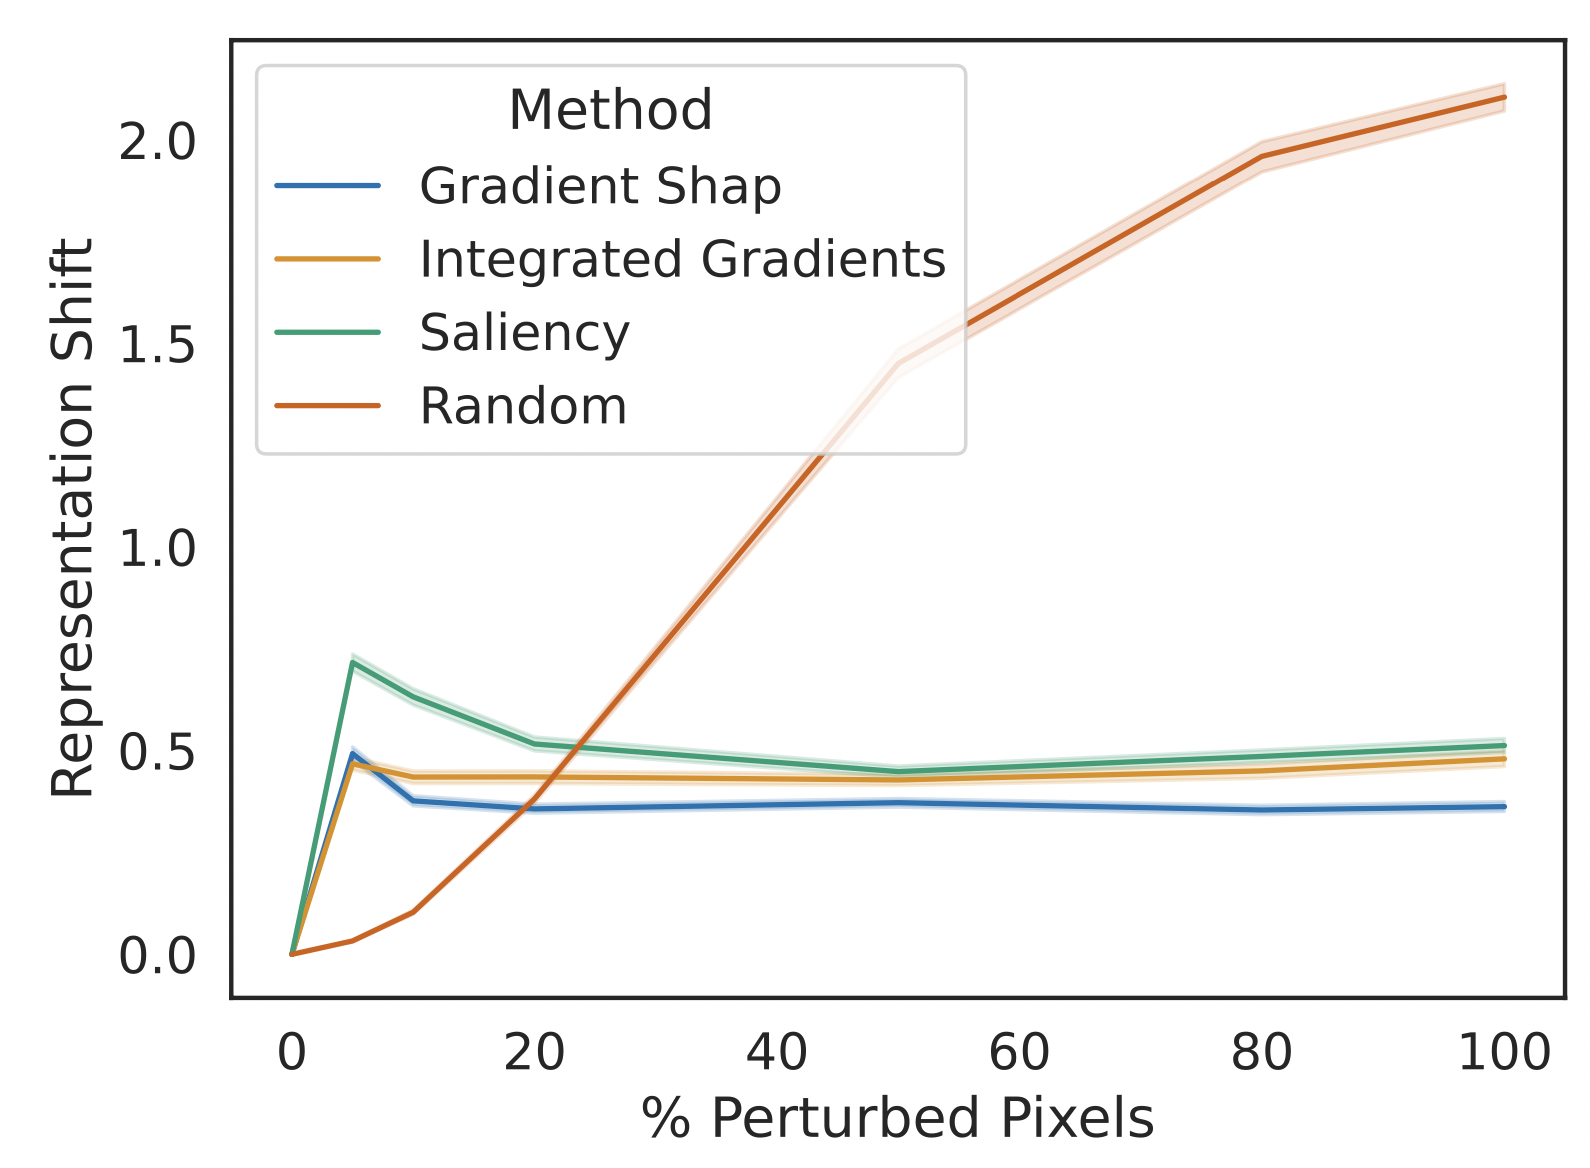
\includegraphics[width=\textwidth]{images/feature_imp/approach2.png} 
\caption{Change in baseline (Equation \ref{eqn:app2})}\label{fig:approach2}
\end{subfigure}
\begin{subfigure}[b]{0.32\linewidth}
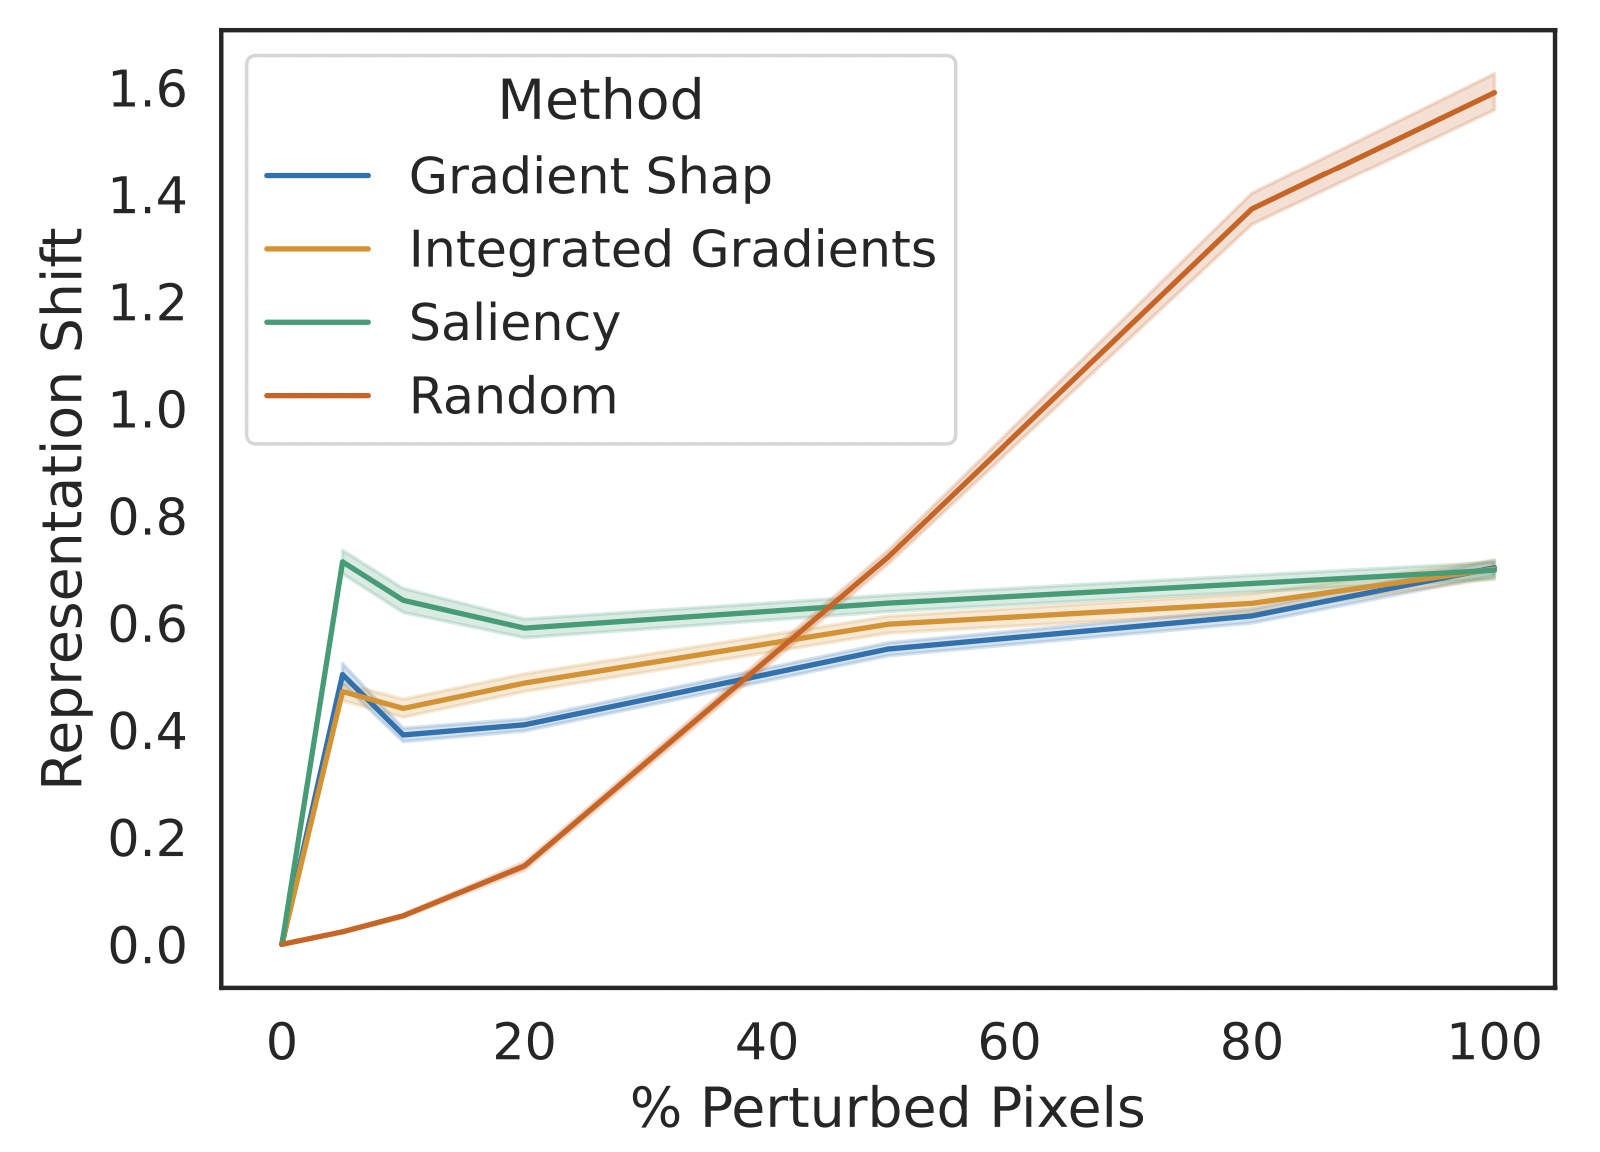
\includegraphics[width=\textwidth]{images/feature_imp/approach3.png} 
\caption{Change in baseline (Equation \ref{eqn:app3})}\label{fig:approach3}
\end{subfigure}
\caption{Consistency check for label-free feature importance (Changes in baseline and masking)}\label{fig:featapproaches}
\end{figure*}


\subsubsection{Result Discussion}
None of the trends (Section \ref{sssec:result1}) in Figure \ref{fig:featapproaches} are satisfied. The shift remains constant for Figures \ref{fig:approach1} and \ref{fig:approach2} after 10\% of perturbations, which suggests that our changes lead to gradient saturation. This leads us to understand why the mask and baselines are assigned values that are independent of the input.


\section{Label Free Example Importance} 
\subsection{Text Explainability}
\label{appendix:textexplain}

\subsubsection{Tokenizer}
\label{sssec:tokenizer_model}
We train a \emph{BertWordPieceTokenizer} model from Huggingface's Tokenizers \citep{tokenizers:online} library using our training texts. We keep the vocabulary size at 10000 while also keeping a minimum token frequency of 2. We then use this trained tokenizer model to tokenize our train and test dataset.

\subsubsection{Model}
\label{sssec:textmodel}

We adapt the architecture for text autoencoder from \citep{torchseq2seq}. Figure \ref{fig:textautoencoderarch} shows an illustration of the final architecture. The layers and their corresponding hyperparameters we use are summarized in Table \ref{tab:text_ae_table}. For our experiments, we keep the latent dimensions (also referred to as context vector) at 128. We use the negative log-likelihood loss (NLLLoss) to train on a number of classes equal to vocabulary size. We also make use of the "Teacher Forcing" concept of using the actual target as inputs to the decoder instead of the last prediction of the decoder, 50\% of the time. We train the model for 8 epochs with a learning rate of 0.01 and a Stochastic Gradient Descent optimizer.

\begin{figure*}[h!]
\centering
    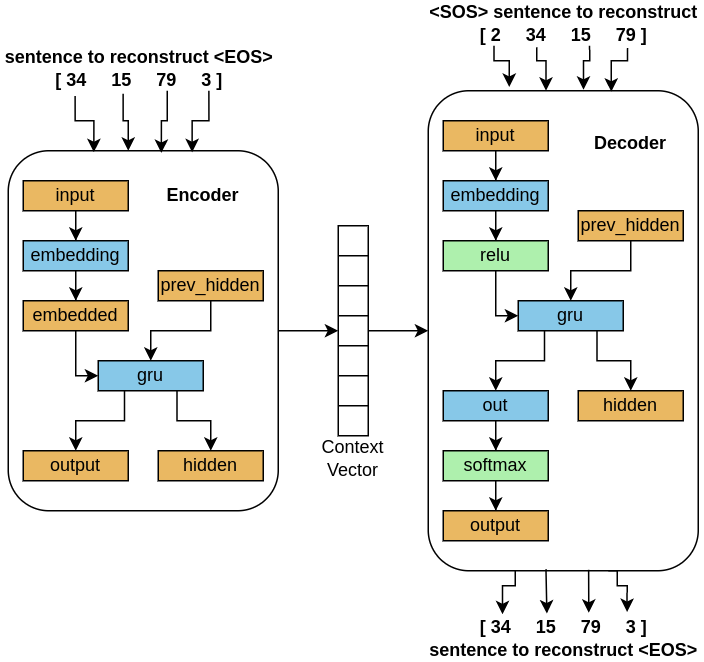
\includegraphics[width=0.7\textwidth]{images/example_imp/text_autoencoder.png}
\caption{Text autoencoder architecture used for text explainability.}\label{fig:textautoencoderarch}
\end{figure*}

\begin{table}[h]
    \small
    \centering
    \begin{tabular}{l|cccc}
    \toprule
    \textbf{Component} & \textbf{Layer Type} & \textbf{Hyperparameters} & \textbf{Act. Func} \\
    \midrule 
    \multirow{2}{*}{Encoder} & Embedding & I/P Feats:10000 ; O/P Feats:128 &  \\
    & GRU &I/P Feats:128 ; O/P Feats:128 &  \\
    \midrule
    \multirow{3}{*}{Decoder}& Embedding & I/P Feats:10000 ; O/P Feats:128 & ReLU \\
    & GRU & I/P Feats:128 ; O/P Feats:128 &  \\
    & Linear & I/P Feats:128 ; O/P Feats:10000 & LogSoftmax \\
    \bottomrule
    \end{tabular}
    \caption{Layers and hyperparameters for text autoencoder model. The last column denotes the activation function used. I/P Feats means Input Features. O/P Feats means output features.}
    \label{tab:text_ae_table}
\end{table}

\newpage
\section{Interpreting the latent units of VAEs with saliency maps}
\subsection{Additional Quantitative Results for Result on Claim 3 - Section \ref{section:result3}}

\begin{figure*}[h!]
\centering
\begin{subfigure}[b]{0.4\linewidth}
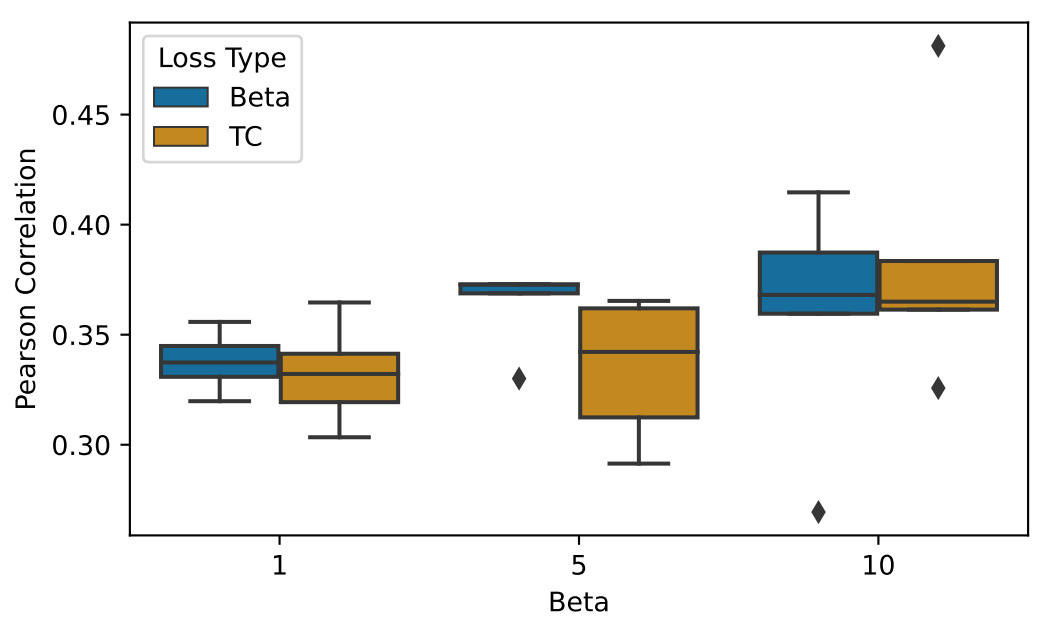
\includegraphics[width=\textwidth]{images/vae/metric_box_plots_mnist_ig.PNG}
\caption{MNIST}\label{fig:metric_box_plots_mnist_ig}
\end{subfigure}
\begin{subfigure}[b]{0.4\linewidth}
\includegraphics[width=\textwidth]{images/vae/metric_box_plots_dSprites_ig.PNG} 
\caption{dSprites}\label{fig:metric_box_plots_dSprites_ig}
\end{subfigure}
\caption{Pearson Correlations over pairs of SM of distinct latent units computed with Integrated Gradients for different values of β.}\label{fig:metrics_plots_extra}
\end{figure*}

\newpage
\subsection{Additional Qualitative Results for Result on Claim 3 - Section \ref{section:result3}}

\begin{figure*}[h]
\centering
    \includegraphics[width=0.7\textwidth]{images/vae/tc_vae_1_sms_dsprites.PNG}
\caption{Saliency maps computed with Gradient Shap from the TC-VAE with  $\beta$=1 on dSprites.}\label{fig:tcvae1smsdsprites}
\end{figure*}

\begin{figure*}[h]
\centering
    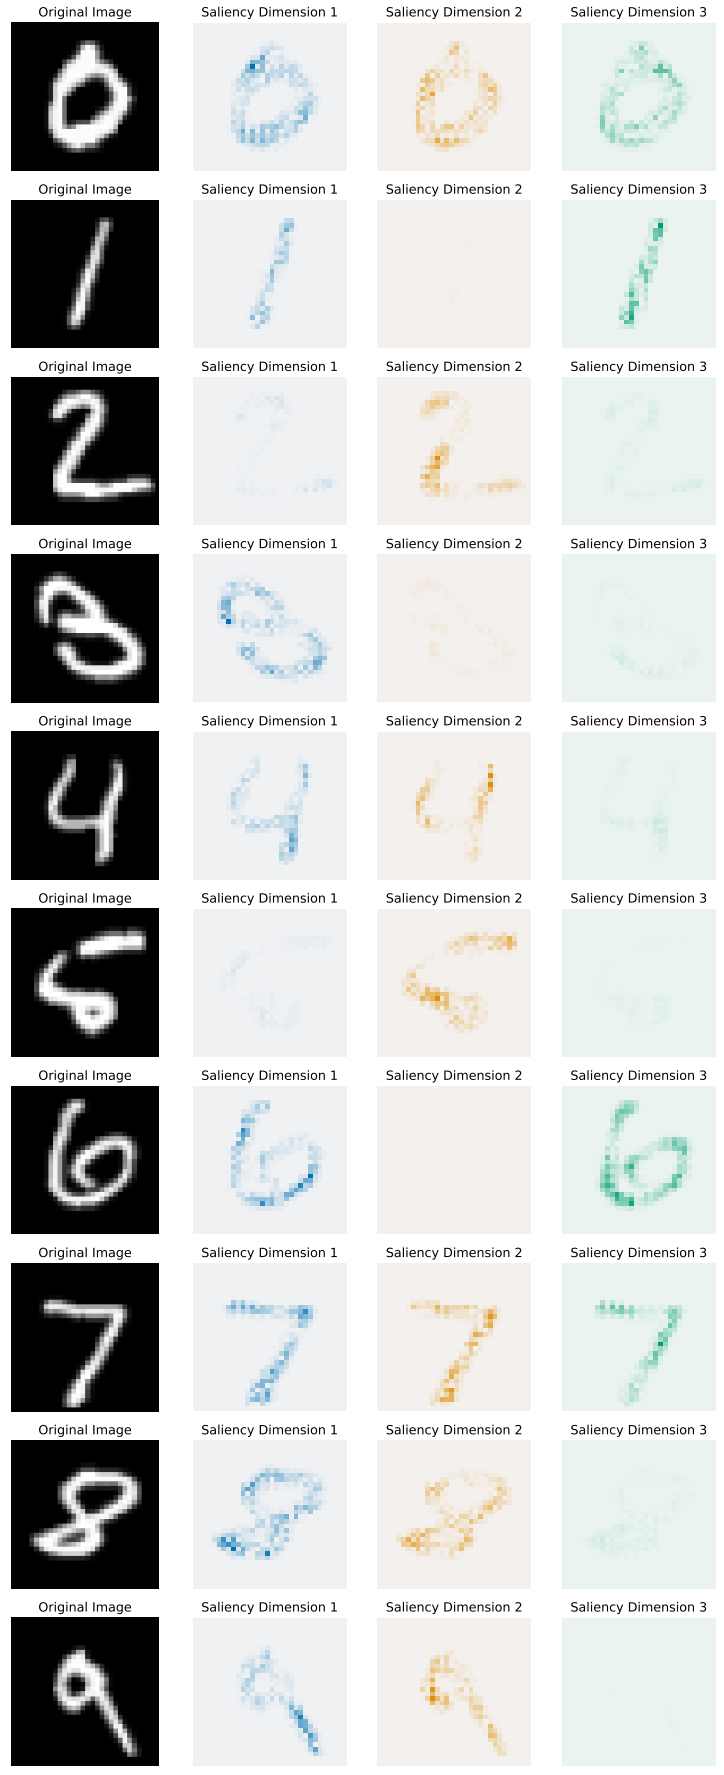
\includegraphics[width=0.7\textwidth]{images/vae/beta_vae_10_sms_mnist_1.PNG}
\caption{Saliency maps computed with Gradient Shap for $\beta$-VAE with  $\beta$=10 on MNIST (Part 1).}\label{fig:betavae10smsmnist1}
\end{figure*}


\begin{figure*}[h]
\centering
    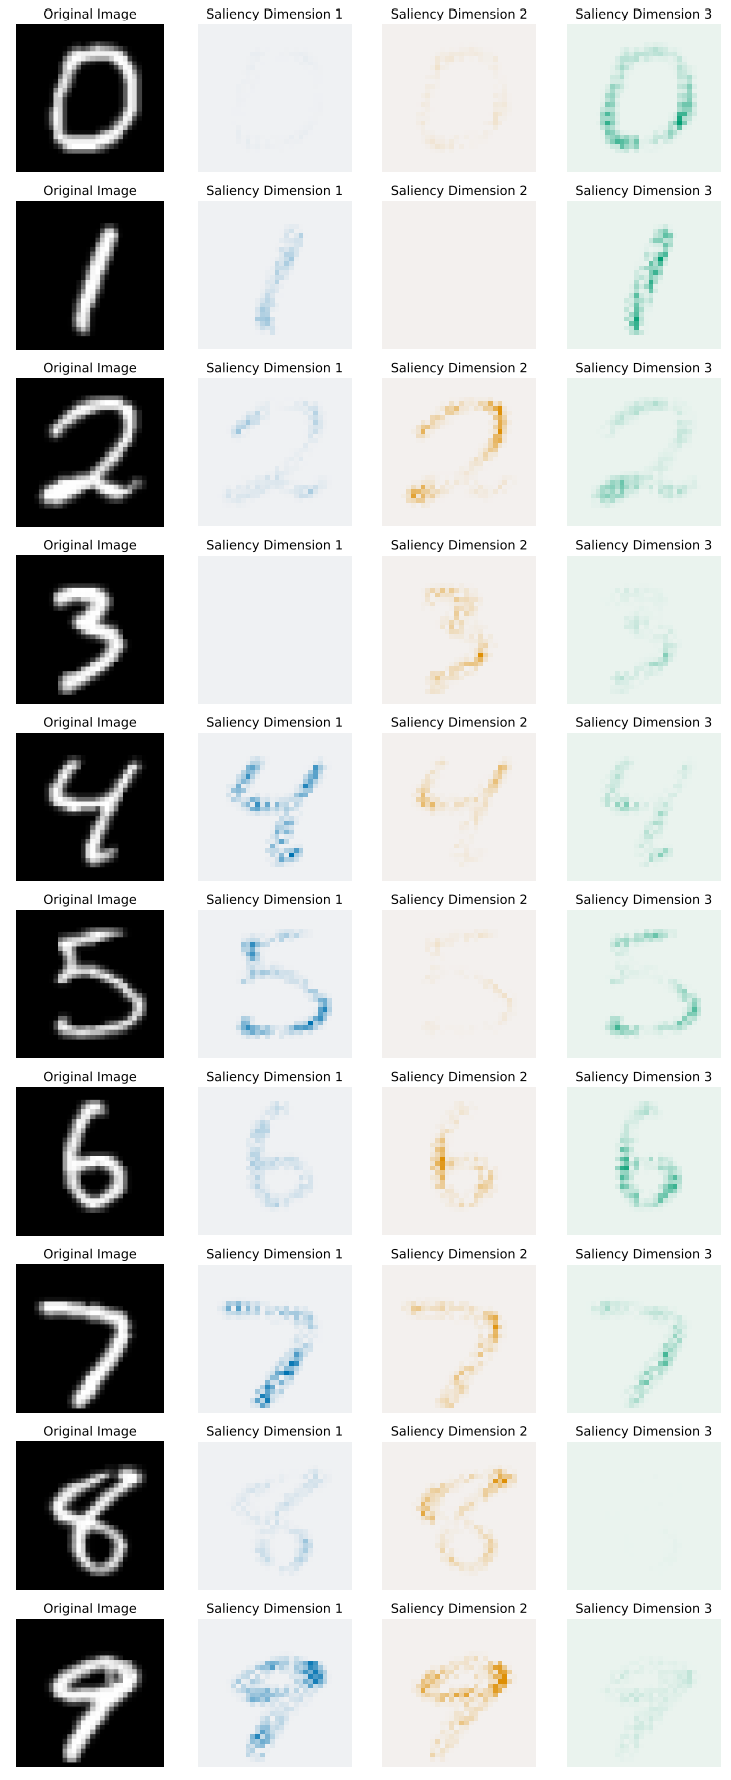
\includegraphics[width=0.7\textwidth]{images/vae/beta_vae_10_sms_mnist_2.PNG}
\caption{Saliency maps computed with Gradient Shap for $\beta$-VAE with  $\beta$=10 on MNIST (Part 2).}\label{fig:betavae10smsmnist2}
\end{figure*}

\clearpage
\subsection{Additional Quantitative Results for Result Section \ref{sec:result3extra}}
\begin{figure*}[h]
\centering
\begin{subfigure}[b]{0.32\linewidth}
\includegraphics[width=\textwidth]{images/vae/metric_box_plots_mnist_0_1.PNG}
\caption{MNIST ($\lambda= 0.1$)}\label{fig:metric_box_plots_mnist_0_1}
\end{subfigure}
\begin{subfigure}[b]{0.32\linewidth}
\includegraphics[width=\textwidth]{images/vae/metric_box_plots_mnist_0_01.PNG}
\caption{MNIST ($\lambda= 0.01$)}\label{fig:metric_box_plots_mnist_0_01}
\end{subfigure}
\begin{subfigure}[b]{0.32\linewidth}
\includegraphics[width=\textwidth]{images/vae/metric_box_plots_mnist_0_001.PNG}
\caption{MNIST ($\lambda= 0.001$)}\label{fig:metric_box_plots_mnist_0_001}
\end{subfigure}
\caption{Pearson Correlations over pairs of SM of distinct latent units with Gradient Shap for different values of β. The models use attribution priors with a regularization parameter, $\lambda$.}\label{fig:attrpriorsboxplts}
\end{figure*}

% these SM Figures of the TC‐VAE with $\beta$=10 and prior attribution to the SM of the $\beta$-VAE with $\beta$=10 and no prior attribution on the MNIST Datasetat from 
\subsection{Additional Qualitative Results for Result Section \ref{sec:result3extra}}\label{app:qualresult3extra}
In Figures \ref{fig:tcvae10smsmnistlambda00011} \& \ref{fig:tc_vae_10_sms_mnist_lambda_0_001_2}, we see the saliency maps (SM) of the latent units of TC‐VAE with $\beta$=10 and $\lambda$=0.001 on the MNIST Dataset. We see figures for $\lambda$=0.005, in Figures \ref{fig:tcvae10smsmnistlambda00051} \& \ref{fig:tcvae10smsmnistlambda00052}. Comparing 
 Figures \ref{fig:betavae10smsmnist1} \& \ref{fig:betavae10smsmnist2}, we see that each latent unit of the TC‐VAE with attribution prior tends to focus on distinct parts of the input image, with less intersection than the latent units of the $\beta$-VAE with no attribution prior. We observe the following cases:
\begin{enumerate}[labelindent=\parindent,leftmargin=*, topsep=0pt]
    \itemsep0em
    \item\label{qualprior:obs1} For the TC‐VAE ($\beta$=10  \& $\lambda$=0.005) in Figure \ref{fig:tcvae10smsmnistlambda00051}, for the digit \textbf{\textit{6}}, latent unit 2 focuses more on the bottom-right part, whereas the latent unit 3 focuses on the top and left part. On the other hand, for the $\beta$-VAE ($\beta$=10 \& no prior) in Figure \ref{fig:betavae10smsmnist1}, the latent units 1 and 3 focus on somewhat different parts of the digit \textbf{\textit{6}}, but there is a significant intersection in the regions they focus on. 
    \item \label{qualprior:obs2}  For the TC‐VAE ($\beta$=10  \& $\lambda$=0.005) in Figure \ref{fig:tcvae10smsmnistlambda00051}, for the digit \textbf{\textit{8}}, latent unit 1 focuses more on the center and upper part of the digit, whereas the latent unit 3 focuses on the bottom part. On the other hand, for the $\beta$-VAE ($\beta$=10 \& no prior) in Figure \ref{fig:betavae10smsmnist1}, the latent units 1 and 2 focus on almost the same regions. 
\end{enumerate}

The observations above seem to be even stronger for the TC‐VAE with $\beta$=10  and smaller $\lambda$ than before, equal to 0.001. Similar observations for SM of the latter model compared to the SM of the $\beta$-VAE with $\beta$=10 and no prior can be made:
\begin{enumerate}[labelindent=\parindent,leftmargin=*, topsep=0pt]
\itemsep0em
    \item\label{qualprior:obs1} For the TC‐VAE ($\beta$=10  \& $\lambda$=0.001) in Figure \ref{fig:tcvae10smsmnistlambda00011}, for the digit \textbf{\textit{4}}, latent unit 1 focuses more on towards the corners and edge-points of the digit
    whereas the latent unit 3 focuses on the vertical main line of the digit \textbf{\textit{4}}. 
    \item\label{qualprior:obs2} For the $\beta$-VAE ($\beta$=10 \& no prior) in Figure \ref{fig:betavae10smsmnist1}, the latent units 1 and 2 focus on somewhat different parts, but there is a significant intersection in the regions they focus on (e.g., the top-right edge-point). 
\end{enumerate}

\bigskip

In conclusion, the prior attribution seems to have the ability to train a model such that its latent units focus on distinct parts with no significant overlapping of the regions they focus on.

\begin{figure*}[h]
\centering
    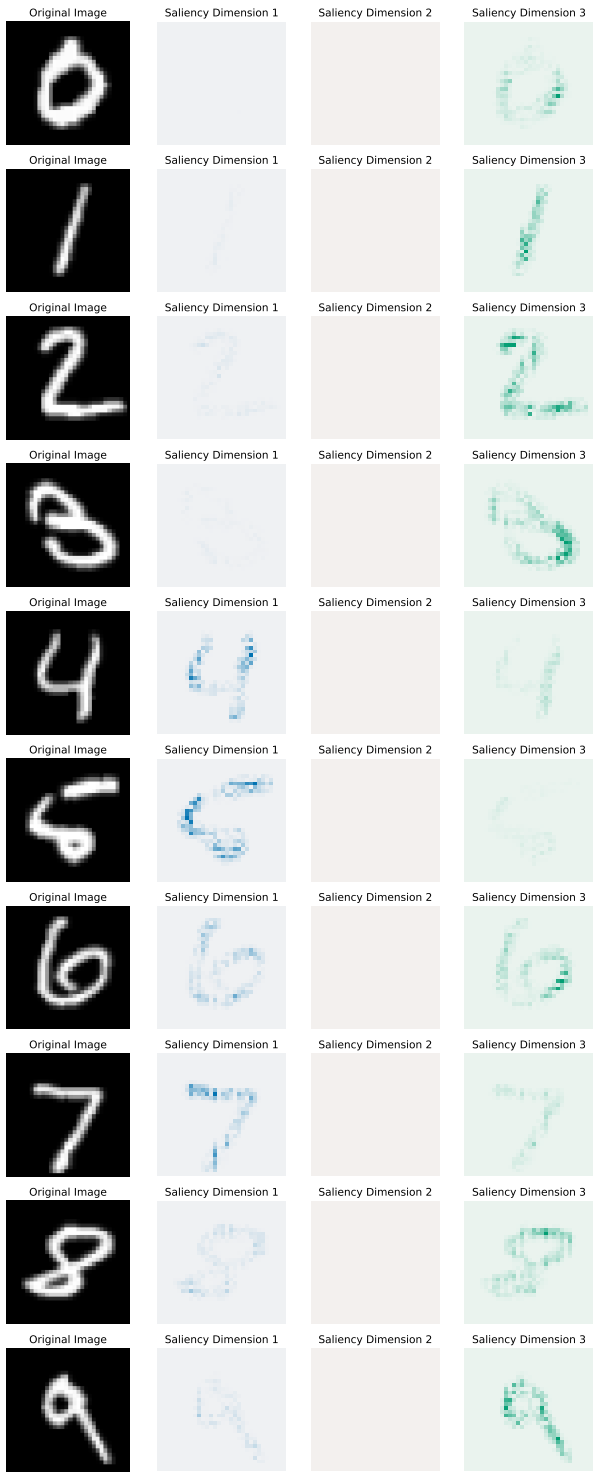
\includegraphics[width=0.7\textwidth]{images/vae/tc_vae_10_sms_mnist_lambda_0_001_1.PNG}
\caption{Saliency maps with Gradient Shap for TC-VAE with  $\beta$=10, $\lambda$=0.001 on MNIST (Part 1).}\label{fig:tcvae10smsmnistlambda00011}
\end{figure*}


\begin{figure*}[h]
\centering
    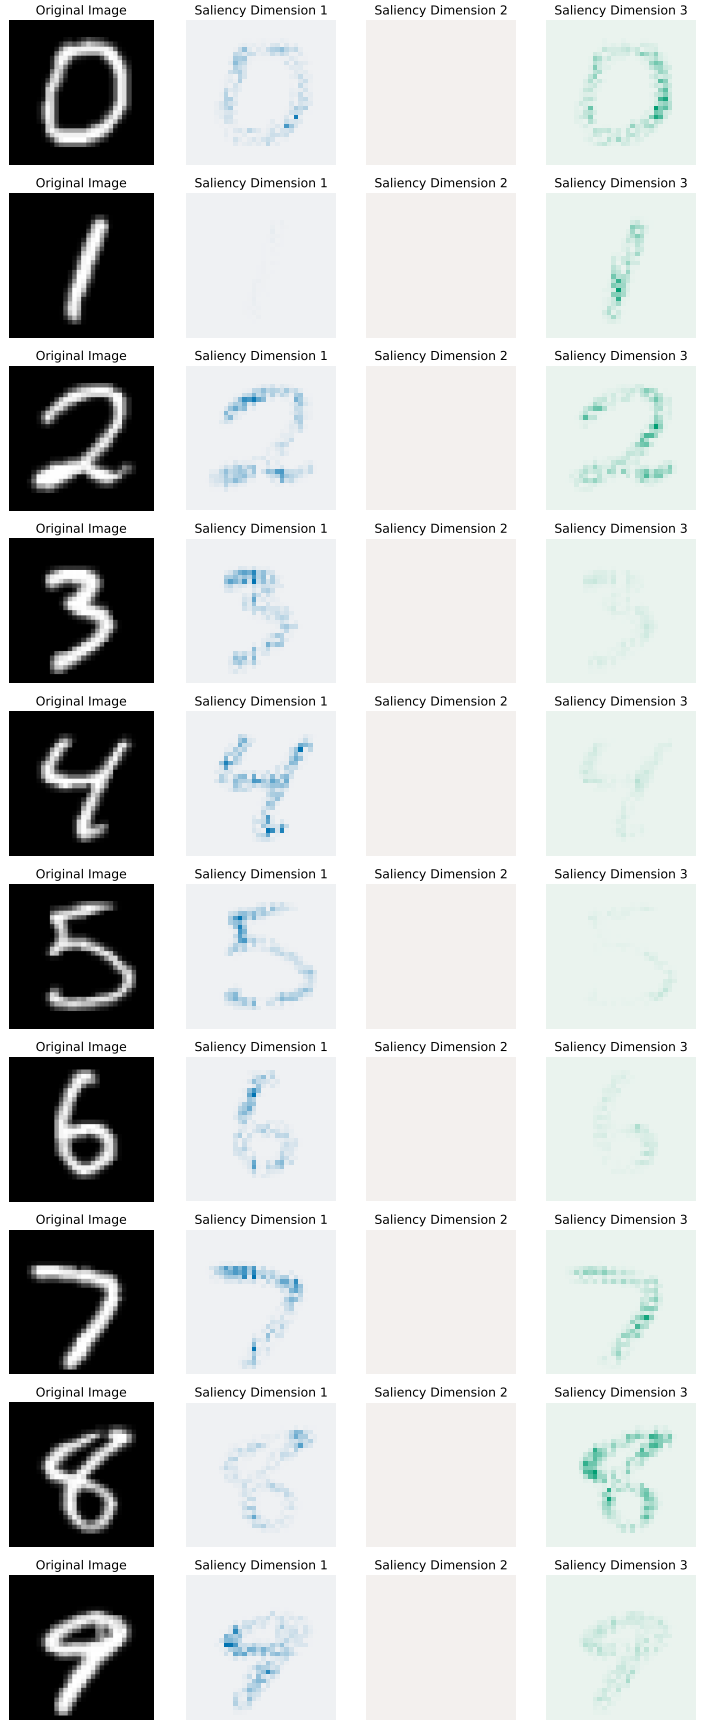
\includegraphics[width=0.7\textwidth]{images/vae/tc_vae_10_sms_mnist_lambda_0_001_2.PNG}
\caption{Saliency maps with Gradient Shap for TC-VAE with  $\beta$=10, $\lambda$=0.001 on MNIST (Part 2).}\label{fig:tc_vae_10_sms_mnist_lambda_0_001_2}
\end{figure*}

\begin{figure*}[h]
\centering
    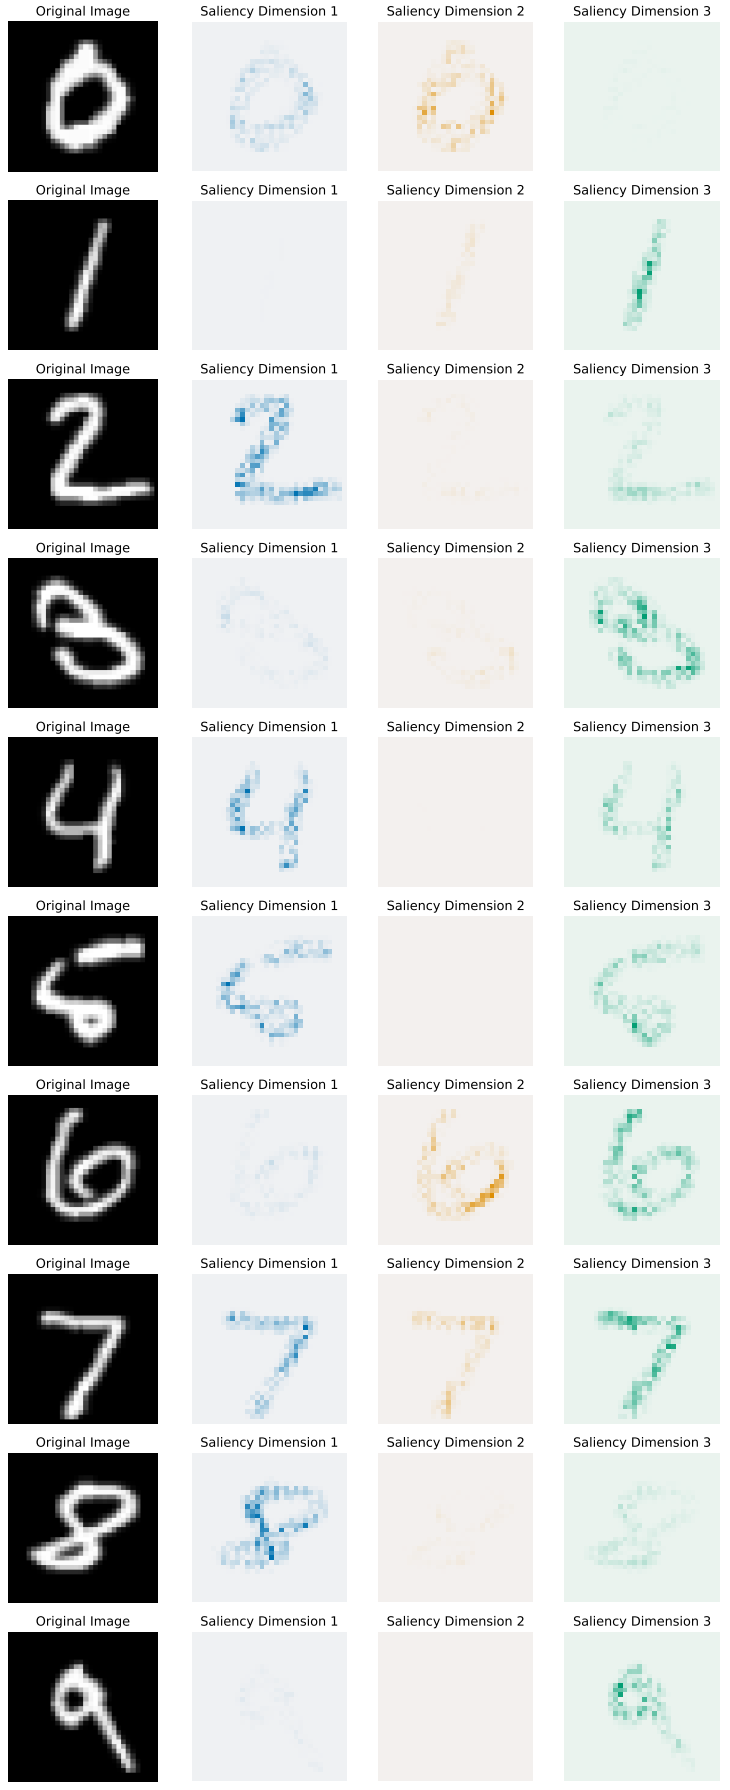
\includegraphics[width=0.7\textwidth]{images/vae/tc_vae_10_sms_mnist_lambda_0_005_1.PNG}
\caption{Saliency maps with Gradient Shap for TC-VAE with  $\beta$=10, $\lambda$=0.005 on MNIST (Part 1).}\label{fig:tcvae10smsmnistlambda00051}
\end{figure*}


\begin{figure*}[h]
\centering
    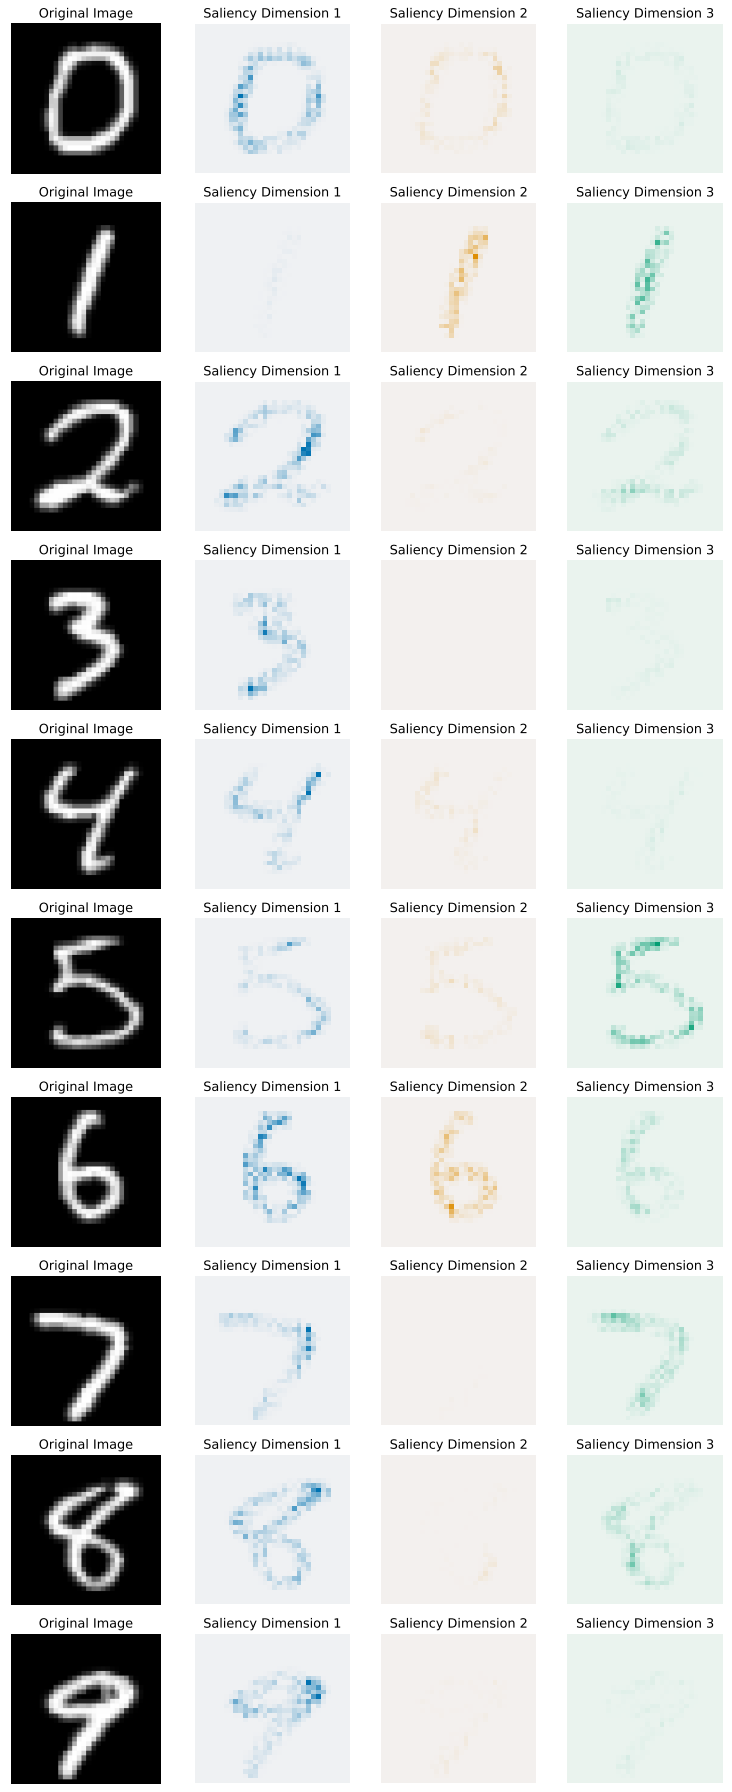
\includegraphics[width=0.7\textwidth]{images/vae/tc_vae_10_sms_mnist_lambda_0_005_2.PNG}
\caption{Saliency maps with Gradient Shap for TC-VAE with  $\beta$=10, $\lambda$=0.005 on MNIST (Part 2).}\label{fig:tcvae10smsmnistlambda00052}
\end{figure*}


\newpage
\clearpage
\subsection{Use Case: Evaluating Label-Free Feature Importance on the Attribution Prior VAEs}
Below you see two tables with the mean (Table \ref{tab:vaespertpercmean}) and standard deviation (Table \ref{tab:vaespertpercstd}) of representation shifts of five runs, for different configurations of models (defined by rows) and different percentages of pixel perturbations applied after training those models (columns 5,10,..., 100) on the MNIST Dataset. The last column shows the test error of the trained model derived from the test set of the MNIST Dataset.

\begin{table}[htbp]
  \centering
    \begin{tabular}{|c|clrrrrrrr|}
    \toprule
    \multicolumn{1}{l}{\textbf{Model}} &
      \multicolumn{1}{l}{\textbf{$\beta$}} &
      \multicolumn{1}{l}{\textbf{$\lambda$}} &
      \textbf{5} &
      \textbf{10} &
      \textbf{20} &
      \textbf{50} &
      \textbf{80} &
      \textbf{100} &
      \multicolumn{1}{l}{\textbf{Test Loss}}
      \\
    \midrule
    \multirow{12}[6]{*}{TC-VAE} &
      \multirow{4}[2]{*}{1} &
      0 &
      \cellcolor[rgb]{ 1,  .937,  .612}0.58 &
      \cellcolor[rgb]{ .957,  .925,  .604}2.84 &
      \cellcolor[rgb]{ .698,  .843,  .549}15.96 &
      \cellcolor[rgb]{ .455,  .769,  .498}28.35 &
      \cellcolor[rgb]{ .455,  .769,  .498}28.35 &
      \cellcolor[rgb]{ .455,  .769,  .498}28.35 &
      176.4
      \\
     &
       &
      0.005 &
      \cellcolor[rgb]{ 1,  .937,  .612}0.65 &
      \cellcolor[rgb]{ .949,  .922,  .604}3.19 &
      \cellcolor[rgb]{ .714,  .847,  .553}15.21 &
      \cellcolor[rgb]{ .514,  .784,  .51}25.4 &
      \cellcolor[rgb]{ .514,  .784,  .51}25.4 &
      \cellcolor[rgb]{ .514,  .784,  .51}25.4 &
      \cellcolor[rgb]{ .608,  .761,  .902}178.8
      \\
     &
       &
      0.01 &
      \cellcolor[rgb]{ 1,  .937,  .612}0.7 &
      \cellcolor[rgb]{ .945,  .922,  .6}3.47 &
      \cellcolor[rgb]{ .659,  .831,  .541}18.05 &
      \cellcolor[rgb]{ .388,  .745,  .482}31.66 &
      \cellcolor[rgb]{ .388,  .745,  .482}31.66 &
      \cellcolor[rgb]{ .388,  .745,  .482}31.66 &
      \cellcolor[rgb]{ .953,  .973,  .988}176.7
      \\
     &
       &
      0.1 &
      \cellcolor[rgb]{ 1,  .937,  .612}0.64 &
      \cellcolor[rgb]{ .957,  .925,  .604}2.94 &
      \cellcolor[rgb]{ .761,  .863,  .565}12.81 &
      \cellcolor[rgb]{ .635,  .824,  .537}19.24 &
      \cellcolor[rgb]{ .635,  .824,  .537}19.24 &
      \cellcolor[rgb]{ .635,  .824,  .537}19.24 &
      \cellcolor[rgb]{ .922,  .953,  .98}176.9
      \\
\cmidrule{2-10}     &
      \multirow{4}[2]{*}{5} &
      0 &
      \cellcolor[rgb]{ 1,  .937,  .612}0.83 &
      \cellcolor[rgb]{ .945,  .922,  .6}2.8 &
      \cellcolor[rgb]{ .773,  .867,  .565}9.08 &
      \cellcolor[rgb]{ .631,  .824,  .537}14.11 &
      \cellcolor[rgb]{ .631,  .824,  .537}14.11 &
      \cellcolor[rgb]{ .631,  .824,  .537}14.11 &
      \cellcolor[rgb]{ .902,  .941,  .976}169.8
      \\
     &
       &
      0.005 &
      \cellcolor[rgb]{ 1,  .937,  .612}0.77 &
      \cellcolor[rgb]{ .945,  .922,  .6}2.83 &
      \cellcolor[rgb]{ .71,  .847,  .553}11.29 &
      \cellcolor[rgb]{ .525,  .788,  .514}17.89 &
      \cellcolor[rgb]{ .525,  .788,  .514}17.89 &
      \cellcolor[rgb]{ .525,  .788,  .514}17.89 &
      \cellcolor[rgb]{ .608,  .761,  .902}172.7
      \\
     &
       &
      0.01 &
      \cellcolor[rgb]{ 1,  .937,  .612}0.84 &
      \cellcolor[rgb]{ .933,  .918,  .6}3.19 &
      \cellcolor[rgb]{ .643,  .827,  .537}13.76 &
      \cellcolor[rgb]{ .388,  .745,  .482}22.8 &
      \cellcolor[rgb]{ .388,  .745,  .482}22.8 &
      \cellcolor[rgb]{ .388,  .745,  .482}22.8 &
      \cellcolor[rgb]{ .98,  .988,  .996}169
      \\
     &
       &
      0.1 &
      \cellcolor[rgb]{ 1,  .937,  .612}0.86 &
      \cellcolor[rgb]{ .953,  .925,  .604}2.49 &
      \cellcolor[rgb]{ .78,  .871,  .569}8.7 &
      \cellcolor[rgb]{ .647,  .827,  .537}13.49 &
      \cellcolor[rgb]{ .647,  .827,  .537}13.49 &
      \cellcolor[rgb]{ .647,  .827,  .537}13.49 &
      168.8
      \\
\cmidrule{2-10}     &
      \multirow{4}[2]{*}{10} &
      0 &
      \cellcolor[rgb]{ .988,  .933,  .612}1.17 &
      \cellcolor[rgb]{ .914,  .91,  .596}3.16 &
      \cellcolor[rgb]{ .671,  .835,  .545}9.73 &
      \cellcolor[rgb]{ .471,  .773,  .502}15.04 &
      \cellcolor[rgb]{ .471,  .773,  .502}15.04 &
      \cellcolor[rgb]{ .471,  .773,  .502}15.04 &
      \cellcolor[rgb]{ .608,  .761,  .902}156.41
      \\
     &
       &
      0.005 &
      \cellcolor[rgb]{ .996,  .937,  .612}0.96 &
      \cellcolor[rgb]{ .925,  .918,  .596}2.79 &
      \cellcolor[rgb]{ .737,  .855,  .557}7.91 &
      \cellcolor[rgb]{ .612,  .816,  .529}11.27 &
      \cellcolor[rgb]{ .612,  .816,  .529}11.27 &
      \cellcolor[rgb]{ .612,  .816,  .529}11.27 &
      154.42
      \\
     &
       &
      0.01 &
      \cellcolor[rgb]{ .996,  .937,  .612}0.95 &
      \cellcolor[rgb]{ .929,  .918,  .6}2.7 &
      \cellcolor[rgb]{ .651,  .827,  .541}10.22 &
      \cellcolor[rgb]{ .388,  .745,  .482}17.21 &
      \cellcolor[rgb]{ .388,  .745,  .482}17.21 &
      \cellcolor[rgb]{ .388,  .745,  .482}17.21 &
      \cellcolor[rgb]{ .706,  .82,  .929}155.93
      \\
     &
       &
      0.1 &
      \cellcolor[rgb]{ 1,  .937,  .612}0.79 &
      \cellcolor[rgb]{ .953,  .922,  .604}2.15 &
      \cellcolor[rgb]{ .773,  .867,  .565}6.9 &
      \cellcolor[rgb]{ .62,  .82,  .533}11.07 &
      \cellcolor[rgb]{ .62,  .82,  .533}11.07 &
      \cellcolor[rgb]{ .62,  .82,  .533}11.07 &
      \cellcolor[rgb]{ .804,  .882,  .953}155.42
      \\
    \midrule
    \multirow{12}[6]{*}{$\beta$-VAE} &
      \multirow{4}[2]{*}{1} &
      0 &
      \cellcolor[rgb]{ .996,  .937,  .612}0.86 &
      \cellcolor[rgb]{ .933,  .918,  .6}5.12 &
      \cellcolor[rgb]{ .631,  .824,  .533}24.97 &
      \cellcolor[rgb]{ .388,  .745,  .482}40.81 &
      \cellcolor[rgb]{ .388,  .745,  .482}40.81 &
      \cellcolor[rgb]{ .388,  .745,  .482}40.81 &
      176.4
      \\
     &
       &
      0.005 &
      \cellcolor[rgb]{ 1,  .937,  .612}0.67 &
      \cellcolor[rgb]{ .961,  .925,  .604}3.11 &
      \cellcolor[rgb]{ .788,  .871,  .569}14.49 &
      \cellcolor[rgb]{ .659,  .831,  .541}23.22 &
      \cellcolor[rgb]{ .659,  .831,  .541}23.22 &
      \cellcolor[rgb]{ .659,  .831,  .541}23.22 &
      \cellcolor[rgb]{ .608,  .761,  .902}178.8
      \\
     &
       &
      0.01 &
      \cellcolor[rgb]{ 1,  .937,  .612}0.6 &
      \cellcolor[rgb]{ .969,  .929,  .608}2.72 &
      \cellcolor[rgb]{ .796,  .875,  .569}14.19 &
      \cellcolor[rgb]{ .627,  .82,  .533}25.28 &
      \cellcolor[rgb]{ .627,  .82,  .533}25.28 &
      \cellcolor[rgb]{ .627,  .82,  .533}25.28 &
      \cellcolor[rgb]{ .953,  .973,  .988}176.7
      \\
     &
       &
      0.1 &
      \cellcolor[rgb]{ 1,  .937,  .612}0.5 &
      \cellcolor[rgb]{ .973,  .929,  .608}2.37 &
      \cellcolor[rgb]{ .839,  .89,  .58}11.14 &
      \cellcolor[rgb]{ .745,  .859,  .561}17.37 &
      \cellcolor[rgb]{ .745,  .859,  .561}17.37 &
      \cellcolor[rgb]{ .745,  .859,  .561}17.37 &
      \cellcolor[rgb]{ .922,  .953,  .98}176.9
      \\
\cmidrule{2-10}     &
      \multirow{4}[2]{*}{5} &
      0 &
      \cellcolor[rgb]{ 1,  .937,  .612}0.85 &
      \cellcolor[rgb]{ .953,  .925,  .604}2.32 &
      \cellcolor[rgb]{ .827,  .886,  .576}6.42 &
      \cellcolor[rgb]{ .749,  .859,  .561}8.92 &
      \cellcolor[rgb]{ .749,  .859,  .561}8.92 &
      \cellcolor[rgb]{ .749,  .859,  .561}8.92 &
      \cellcolor[rgb]{ .902,  .941,  .976}169.8
      \\
     &
       &
      0.005 &
      \cellcolor[rgb]{ 1,  .937,  .612}0.8 &
      \cellcolor[rgb]{ .941,  .922,  .6}2.76 &
      \cellcolor[rgb]{ .647,  .827,  .537}12.27 &
      \cellcolor[rgb]{ .388,  .745,  .482}20.62 &
      \cellcolor[rgb]{ .388,  .745,  .482}20.62 &
      \cellcolor[rgb]{ .388,  .745,  .482}20.62 &
      \cellcolor[rgb]{ .608,  .761,  .902}172.7
      \\
     &
       &
      0.01 &
      \cellcolor[rgb]{ .992,  .937,  .612}1.07 &
      \cellcolor[rgb]{ .918,  .914,  .596}3.53 &
      \cellcolor[rgb]{ .671,  .835,  .545}11.5 &
      \cellcolor[rgb]{ .506,  .784,  .51}16.82 &
      \cellcolor[rgb]{ .506,  .784,  .51}16.82 &
      \cellcolor[rgb]{ .506,  .784,  .51}16.82 &
      \cellcolor[rgb]{ .98,  .988,  .996}169
      \\
     &
       &
      0.1 &
      \cellcolor[rgb]{ 1,  .937,  .612}0.75 &
      \cellcolor[rgb]{ .953,  .925,  .604}2.37 &
      \cellcolor[rgb]{ .773,  .867,  .565}8.15 &
      \cellcolor[rgb]{ .624,  .82,  .533}13.01 &
      \cellcolor[rgb]{ .624,  .82,  .533}13.01 &
      \cellcolor[rgb]{ .624,  .82,  .533}13.01 &
      168.8
      \\
\cmidrule{2-10}     &
      \multirow{4}[2]{*}{10} &
      0 &
      \cellcolor[rgb]{ 1,  .937,  .612}0.51 &
      \cellcolor[rgb]{ .929,  .918,  .596}1.34 &
      \cellcolor[rgb]{ .639,  .827,  .537}4.55 &
      \cellcolor[rgb]{ .388,  .745,  .482}7.35 &
      \cellcolor[rgb]{ .388,  .745,  .482}7.35 &
      \cellcolor[rgb]{ .388,  .745,  .482}7.35 &
      \cellcolor[rgb]{ .608,  .761,  .902}156.41
      \\
     &
       &
      0.005 &
      \cellcolor[rgb]{ .984,  .933,  .608}0.72 &
      \cellcolor[rgb]{ .871,  .898,  .584}1.97 &
      \cellcolor[rgb]{ .608,  .816,  .529}4.93 &
      \cellcolor[rgb]{ .475,  .773,  .502}6.4 &
      \cellcolor[rgb]{ .475,  .773,  .502}6.4 &
      \cellcolor[rgb]{ .475,  .773,  .502}6.4 &
      154.42
      \\
     &
       &
      0.01 &
      \cellcolor[rgb]{ .984,  .933,  .612}0.7 &
      \cellcolor[rgb]{ .886,  .902,  .588}1.8 &
      \cellcolor[rgb]{ .655,  .831,  .541}4.4 &
      \cellcolor[rgb]{ .506,  .784,  .51}6.07 &
      \cellcolor[rgb]{ .506,  .784,  .51}6.07 &
      \cellcolor[rgb]{ .506,  .784,  .51}6.07 &
      \cellcolor[rgb]{ .706,  .82,  .929}155.93
      \\
     &
       &
      0.1 &
      \cellcolor[rgb]{ .992,  .937,  .612}0.63 &
      \cellcolor[rgb]{ .91,  .91,  .592}1.56 &
      \cellcolor[rgb]{ .714,  .851,  .553}3.72 &
      \cellcolor[rgb]{ .608,  .816,  .529}4.92 &
      \cellcolor[rgb]{ .608,  .816,  .529}4.92 &
      \cellcolor[rgb]{ .608,  .816,  .529}4.92 &
      \cellcolor[rgb]{ .804,  .882,  .953}155.42
      \\
    \bottomrule
    \end{tabular}%
  \caption{Mean representation shifts over 5 runs for percentages of pixel perturbations for the models $\beta$-VAE, and TC-VAE on the MNIST dataset with different disentanglement factor $\beta$ and different regularization parameter, $\lambda$. The $\lambda$ is for weighting the importance of the attribution prior to the model's loss function (See Equation \ref{eqn:pixelattrprior}). $\lambda=0$ denotes that no attribution prior is used. The Test Loss is the loss of the model reconstructing the MNIST test dataset. The numbers 5,10,..., 100 represent the percentage of the important pixels of each input image perturbed.}
  \label{tab:vaespertpercmean}%
\end{table}%

% different regularization parameters (=reg)


\clearpage
\newpage
% Table generated by Excel2LaTeX from sheet 'grad_false_std_tex'
\begin{table}[htbp]
  \centering
    \begin{tabular}{|c|clrrrrrr|}
    \toprule
    \multicolumn{1}{l}{\textbf{Model}} &
      \multicolumn{1}{l}{\textbf{$\beta$}} &
      \multicolumn{1}{l}{\textbf{$\lambda$}} &
      \textbf{5} &
      \textbf{10} &
      \textbf{20} &
      \textbf{50} &
      \textbf{80} &
      \multicolumn{1}{r}{100}
      \\
    \midrule
    \multirow{12}[6]{*}{\textbf{TC-VAE}} &
      \multirow{4}[2]{*}{1} &
      0 &
      \cellcolor[rgb]{ .969,  .929,  .608}0.35 &
      \cellcolor[rgb]{ .78,  .871,  .569}1.45 &
      \cellcolor[rgb]{ .388,  .745,  .482}3.75 &
      \cellcolor[rgb]{ .855,  .894,  .584}1.03 &
      \cellcolor[rgb]{ .855,  .894,  .584}1.03 &
      \cellcolor[rgb]{ .855,  .894,  .584}1.03
      \\
     &
       &
      0.005 &
      \cellcolor[rgb]{ .992,  .937,  .612}0.22 &
      \cellcolor[rgb]{ .89,  .906,  .592}0.81 &
      \cellcolor[rgb]{ .718,  .851,  .553}1.83 &
      \cellcolor[rgb]{ .804,  .878,  .573}1.32 &
      \cellcolor[rgb]{ .804,  .878,  .573}1.32 &
      \cellcolor[rgb]{ .804,  .878,  .573}1.32
      \\
     &
       &
      0.01 &
      \cellcolor[rgb]{ 1,  .937,  .612}0.18 &
      \cellcolor[rgb]{ .91,  .91,  .596}0.7 &
      \cellcolor[rgb]{ .655,  .831,  .541}2.19 &
      \cellcolor[rgb]{ .698,  .843,  .549}1.95 &
      \cellcolor[rgb]{ .698,  .843,  .549}1.95 &
      \cellcolor[rgb]{ .698,  .843,  .549}1.95
      \\
     &
       &
      0.1 &
      \cellcolor[rgb]{ 1,  .937,  .612}0.16 &
      \cellcolor[rgb]{ .925,  .914,  .596}0.62 &
      \cellcolor[rgb]{ .776,  .867,  .565}1.49 &
      \cellcolor[rgb]{ .769,  .867,  .565}1.52 &
      \cellcolor[rgb]{ .769,  .867,  .565}1.52 &
      \cellcolor[rgb]{ .769,  .867,  .565}1.52
      \\
\cmidrule{2-9}     &
      \multirow{4}[2]{*}{5} &
      0 &
      \cellcolor[rgb]{ .992,  .937,  .612}0.16 &
      \cellcolor[rgb]{ .922,  .914,  .596}0.35 &
      \cellcolor[rgb]{ .761,  .863,  .561}0.78 &
      \cellcolor[rgb]{ .749,  .859,  .561}0.81 &
      \cellcolor[rgb]{ .749,  .859,  .561}0.81 &
      \cellcolor[rgb]{ .749,  .859,  .561}0.81
      \\
     &
       &
      0.005 &
      \cellcolor[rgb]{ .996,  .937,  .612}0.15 &
      \cellcolor[rgb]{ .847,  .89,  .58}0.55 &
      \cellcolor[rgb]{ .388,  .745,  .482}1.78 &
      \cellcolor[rgb]{ .635,  .824,  .537}1.12 &
      \cellcolor[rgb]{ .635,  .824,  .537}1.12 &
      \cellcolor[rgb]{ .635,  .824,  .537}1.12
      \\
     &
       &
      0.01 &
      \cellcolor[rgb]{ .957,  .925,  .604}0.25 &
      \cellcolor[rgb]{ .796,  .875,  .569}0.69 &
      \cellcolor[rgb]{ .522,  .788,  .51}1.43 &
      \cellcolor[rgb]{ .69,  .843,  .549}0.97 &
      \cellcolor[rgb]{ .69,  .843,  .549}0.97 &
      \cellcolor[rgb]{ .69,  .843,  .549}0.97
      \\
     &
       &
      0.1 &
      \cellcolor[rgb]{ 1,  .937,  .612}0.13 &
      \cellcolor[rgb]{ .914,  .91,  .596}0.37 &
      \cellcolor[rgb]{ .635,  .824,  .537}1.12 &
      \cellcolor[rgb]{ .761,  .863,  .561}0.78 &
      \cellcolor[rgb]{ .761,  .863,  .561}0.78 &
      \cellcolor[rgb]{ .761,  .863,  .561}0.78
      \\
\cmidrule{2-9}     &
      \multirow{4}[2]{*}{10} &
      0 &
      \cellcolor[rgb]{ .98,  .933,  .608}0.1 &
      \cellcolor[rgb]{ .816,  .878,  .573}0.27 &
      \cellcolor[rgb]{ .388,  .745,  .482}0.7 &
      \cellcolor[rgb]{ .675,  .835,  .545}0.41 &
      \cellcolor[rgb]{ .675,  .835,  .545}0.41 &
      \cellcolor[rgb]{ .675,  .835,  .545}0.41
      \\
     &
       &
      0.005 &
      \cellcolor[rgb]{ 1,  .937,  .612}0.08 &
      \cellcolor[rgb]{ .882,  .902,  .588}0.2 &
      \cellcolor[rgb]{ .576,  .808,  .525}0.51 &
      \cellcolor[rgb]{ .627,  .82,  .533}0.46 &
      \cellcolor[rgb]{ .627,  .82,  .533}0.46 &
      \cellcolor[rgb]{ .627,  .82,  .533}0.46
      \\
     &
       &
      0.01 &
      \cellcolor[rgb]{ .98,  .933,  .608}0.1 &
      \cellcolor[rgb]{ .855,  .894,  .584}0.23 &
      \cellcolor[rgb]{ .569,  .804,  .522}0.52 &
      \cellcolor[rgb]{ .718,  .851,  .553}0.37 &
      \cellcolor[rgb]{ .718,  .851,  .553}0.37 &
      \cellcolor[rgb]{ .718,  .851,  .553}0.37
      \\
     &
       &
      0.1 &
      \cellcolor[rgb]{ 1,  .937,  .612}0.08 &
      \cellcolor[rgb]{ .875,  .898,  .588}0.21 &
      \cellcolor[rgb]{ .694,  .843,  .549}0.39 &
      \cellcolor[rgb]{ .718,  .851,  .553}0.37 &
      \cellcolor[rgb]{ .718,  .851,  .553}0.37 &
      \cellcolor[rgb]{ .718,  .851,  .553}0.37
      \\
    \midrule
    \multirow{12}[6]{*}{$\beta$-VAE} &
      \multirow{4}[2]{*}{1} &
      0 &
      \cellcolor[rgb]{ 1,  .937,  .612}0.18 &
      \cellcolor[rgb]{ .855,  .894,  .58}0.8 &
      \cellcolor[rgb]{ .447,  .765,  .494}2.5 &
      \cellcolor[rgb]{ .686,  .839,  .545}1.5 &
      \cellcolor[rgb]{ .686,  .839,  .545}1.5 &
      \cellcolor[rgb]{ .686,  .839,  .545}1.5
      \\
     &
       &
      0.005 &
      \cellcolor[rgb]{ .992,  .937,  .612}0.22 &
      \cellcolor[rgb]{ .843,  .89,  .58}0.85 &
      \cellcolor[rgb]{ .522,  .788,  .514}2.18 &
      \cellcolor[rgb]{ .733,  .855,  .557}1.3 &
      \cellcolor[rgb]{ .733,  .855,  .557}1.3 &
      \cellcolor[rgb]{ .733,  .855,  .557}1.3
      \\
     &
       &
      0.01 &
      \cellcolor[rgb]{ .992,  .937,  .612}0.22 &
      \cellcolor[rgb]{ .812,  .878,  .573}0.98 &
      \cellcolor[rgb]{ .388,  .745,  .482}2.73 &
      \cellcolor[rgb]{ .565,  .8,  .522}2.01 &
      \cellcolor[rgb]{ .565,  .8,  .522}2.01 &
      \cellcolor[rgb]{ .565,  .8,  .522}2.01
      \\
     &
       &
      0.1 &
      \cellcolor[rgb]{ .992,  .937,  .612}0.22 &
      \cellcolor[rgb]{ .847,  .89,  .58}0.82 &
      \cellcolor[rgb]{ .655,  .831,  .541}1.62 &
      \cellcolor[rgb]{ .733,  .855,  .557}1.3 &
      \cellcolor[rgb]{ .733,  .855,  .557}1.3 &
      \cellcolor[rgb]{ .733,  .855,  .557}1.3
      \\
\cmidrule{2-9}     &
      \multirow{4}[2]{*}{5} &
      0 &
      \cellcolor[rgb]{ .98,  .933,  .608}0.21 &
      \cellcolor[rgb]{ .878,  .902,  .588}0.55 &
      \cellcolor[rgb]{ .686,  .839,  .549}1.21 &
      \cellcolor[rgb]{ .808,  .878,  .573}0.8 &
      \cellcolor[rgb]{ .808,  .878,  .573}0.8 &
      \cellcolor[rgb]{ .808,  .878,  .573}0.8
      \\
     &
       &
      0.005 &
      \cellcolor[rgb]{ .976,  .929,  .608}0.22 &
      \cellcolor[rgb]{ .835,  .886,  .58}0.7 &
      \cellcolor[rgb]{ .502,  .784,  .51}1.84 &
      \cellcolor[rgb]{ .784,  .871,  .569}0.88 &
      \cellcolor[rgb]{ .784,  .871,  .569}0.88 &
      \cellcolor[rgb]{ .784,  .871,  .569}0.88
      \\
     &
       &
      0.01 &
      \cellcolor[rgb]{ .984,  .933,  .612}0.19 &
      \cellcolor[rgb]{ .831,  .886,  .576}0.72 &
      \cellcolor[rgb]{ .388,  .745,  .482}2.23 &
      \cellcolor[rgb]{ .694,  .843,  .549}1.19 &
      \cellcolor[rgb]{ .694,  .843,  .549}1.19 &
      \cellcolor[rgb]{ .694,  .843,  .549}1.19
      \\
     &
       &
      0.1 &
      \cellcolor[rgb]{ 1,  .937,  .612}0.13 &
      \cellcolor[rgb]{ .925,  .914,  .596}0.39 &
      \cellcolor[rgb]{ .733,  .855,  .557}1.05 &
      \cellcolor[rgb]{ .584,  .808,  .525}1.57 &
      \cellcolor[rgb]{ .584,  .808,  .525}1.57 &
      \cellcolor[rgb]{ .584,  .808,  .525}1.57
      \\
\cmidrule{2-9}     &
      \multirow{4}[2]{*}{10} &
      0 &
      \cellcolor[rgb]{ .961,  .925,  .604}0.29 &
      \cellcolor[rgb]{ .839,  .886,  .58}0.67 &
      \cellcolor[rgb]{ .502,  .78,  .51}1.72 &
      \cellcolor[rgb]{ .749,  .859,  .561}0.95 &
      \cellcolor[rgb]{ .749,  .859,  .561}0.95 &
      \cellcolor[rgb]{ .749,  .859,  .561}0.95
      \\
     &
       &
      0.005 &
      \cellcolor[rgb]{ .992,  .937,  .612}0.19 &
      \cellcolor[rgb]{ .906,  .91,  .592}0.46 &
      \cellcolor[rgb]{ .733,  .855,  .557}1 &
      \cellcolor[rgb]{ .847,  .89,  .58}0.64 &
      \cellcolor[rgb]{ .847,  .89,  .58}0.64 &
      \cellcolor[rgb]{ .847,  .89,  .58}0.64
      \\
     &
       &
      0.01 &
      \cellcolor[rgb]{ .996,  .937,  .612}0.18 &
      \cellcolor[rgb]{ .875,  .898,  .588}0.56 &
      \cellcolor[rgb]{ .388,  .745,  .482}2.07 &
      \cellcolor[rgb]{ .616,  .82,  .533}1.36 &
      \cellcolor[rgb]{ .616,  .82,  .533}1.36 &
      \cellcolor[rgb]{ .616,  .82,  .533}1.36
      \\
     &
       &
      0.1 &
      \cellcolor[rgb]{ 1,  .937,  .612}0.16 &
      \cellcolor[rgb]{ .929,  .918,  .6}0.39 &
      \cellcolor[rgb]{ .655,  .831,  .541}1.24 &
      \cellcolor[rgb]{ .694,  .843,  .549}1.12 &
      \cellcolor[rgb]{ .694,  .843,  .549}1.12 &
      \cellcolor[rgb]{ .694,  .843,  .549}1.12
      \\
    \bottomrule
    \end{tabular}%
  \caption{ Standard Deviation of the representation shifts over 5 runs for Table \ref{tab:vaespertpercmean}. 
  }
\label{tab:vaespertpercstd}%
\end{table}%



\section{Representations Learnt on Pretext Tasks}
\vspace{-1mm}
\subsection{Qualitative analysis overview}
\label{app:qualitativeanalysis}
    We perform an extensive qualitative analysis by comparing the output saliency maps and top examples. Below in this section, we include figures of some notable cases of top examples and their saliency maps. Multiple groups of images are collected for different runs on the dataset. 
    
    In the case of the saliency maps, it is indeed true that for the same image, there are notable differences across different pretext tasks, since the highlighted regions are not the same. On the other hand, in the case of example importance the conclusion that \enquote{the top examples are rarely similar across various pretext tasks} does not coincide with the observations of the reproduced outputs. As seen in Figure \ref{app:SMs}, most of the top examples correspond to the right number, although in some images they do not coincide. Finally, we observe the synergy between the top examples and the feature importance. 
    \vspace{-2mm}
    \begin{table}[H]
    \centering
    \label{tab:qualitativeanalysis}
    \begin{tabular}{l|l}
    \hline
     \textbf{Qualitative claim}  & \textbf{Status} \\  
     \hline 
     Saliency maps differences  & Confirmed \\
     Top example differences & Unconfirmed \\
     Synergy   & Confirmed \\           
    \hline
      
\end{tabular}
  \caption{Qualitative analysis}
\end{table}

    \begin{figure}
        \centering
        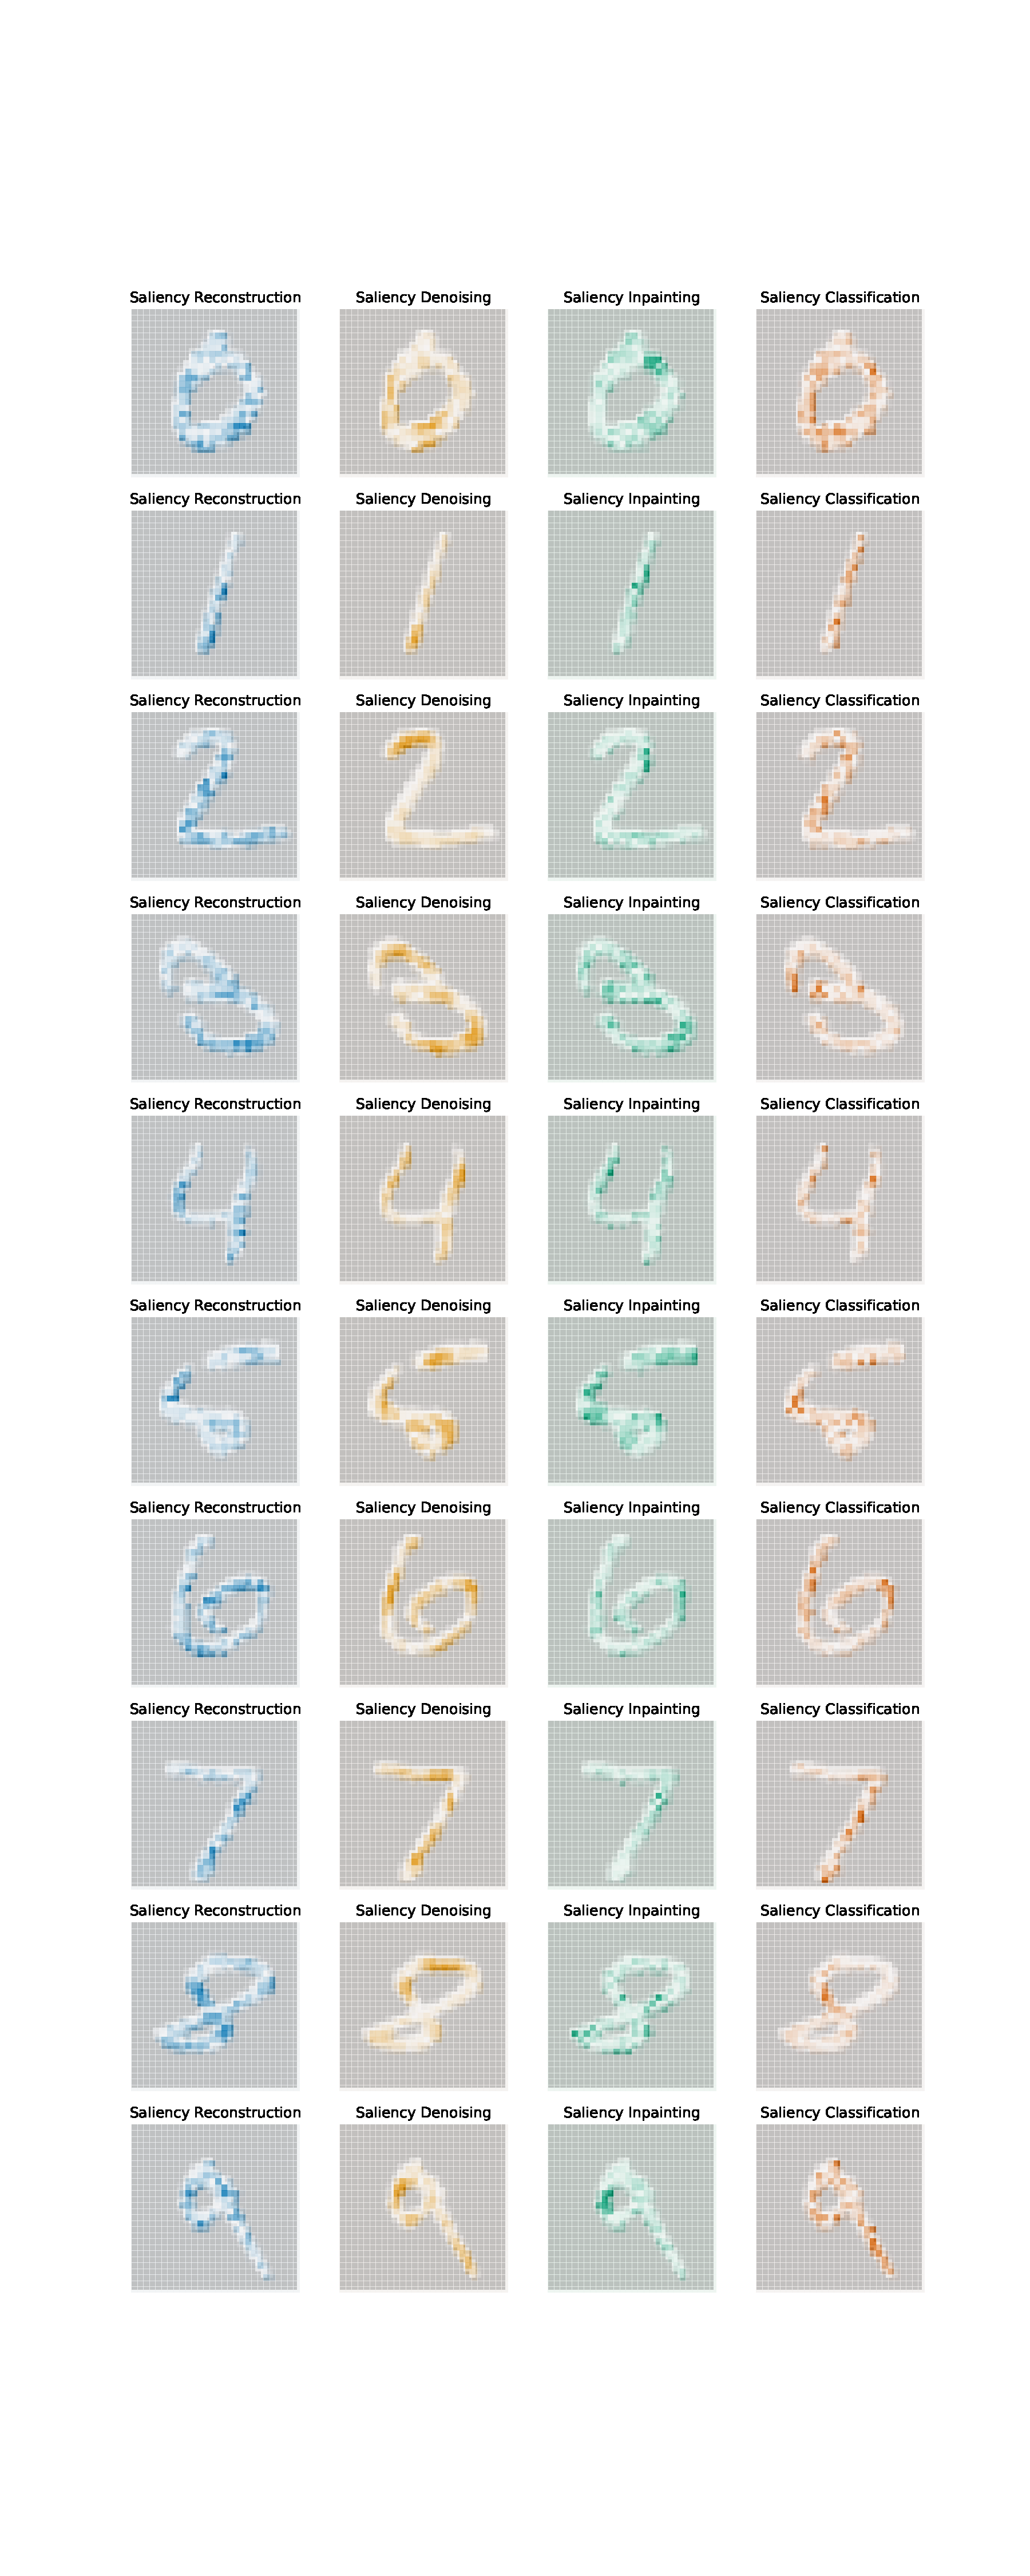
\includegraphics[width=0.7\textwidth]{images/example_imp/saliency_maps_run0.pdf}
        \caption{Reproduced label-free saliency maps for various pretext tasks (Run 0)}
        \label{app:SMs}
    \end{figure}

\newpage

    \begin{figure}
        \centering
        \includegraphics[width=0.75\textwidth]{images/feature_imp/top_examples_run0.pdf}
        \caption{Reproduced label-free top examples for various pretext tasks (Run 0)}
        \label{fig:my_label}
    \end{figure}

    